%%%%%%%%%%%%%%%%%%%%%%%%%%%%%%%
% COM3502-4502-6502 Speech Processing
% Main Programming Assignment Response Sheet
% Prof. Roger K. Moore
% University of Sheffield
% 31 October 2019
%%%%%%%%%%%%%%%%%%%%%%%%%%%%%%%

\documentclass[hidelinks,a4paper,11pt]{article}

\usepackage[margin=1.2in]{geometry}
\usepackage{graphicx}
\usepackage{hyperref}
\usepackage[parfill]{parskip}
\usepackage{mdframed}
\usepackage{enumitem,amssymb}
\usepackage{float}
\newcounter{question}
\newcommand\myq{\refstepcounter{question}\thequestion}
\usepackage{gensymb}
\usepackage{tipa}  % IPA symbols
\usepackage[bottom]{footmisc}


\begin{document}

\begin{titlepage}

\begin{center}
{\LARGE University of Sheffield}\\[1cm]
\huge {\bfseries COM3502-4502-6502\\Speech Processing}\\[1cm]

\includegraphics[width=5cm]{tuoslogo.png}\\[1cm]
{\huge \bfseries Main Programming Assignment}\\[0.5cm]

%vvvvvvvvvvvvvvvvvvvvvvvvvvvvvvvvvvvvvvvvvvvvvvvvvvvvvvvvvvvvvv
% EDIT YOUR NAMES
{\Large Simon Fish}\\
{\Large Zheming Qiu}\\[1cm]
%^^^^^^^^^^^^^^^^^^^^^^^^^^^^^^^^^^^^^^^^^^^^^^^^^^^^^^^^^^^^^^^^^^

{\LARGE Department of Computer Science}\\
{\Large \today}
\end{center}

\end{titlepage}

{\color{red}{\bfseries QUESTION \myq\ \emph{(worth up to 5 marks)}}\\Provide a screenshot of \texttt{[wsprobe$\sim$]} for a typical voiced sound, and explain the features in the waveform and spectrum that distinguish it from an unvoiced sound.  \emph{Hint: use the `snapshot' feature in \texttt{[wsprobe$\sim$]} to obtain a static display.}}
\\
\begin{mdframed}
\emph{"m" in word "midnight" screenshotted below.} \\
The waveform is much noisier for unvoiced sounds like "s". The spectrum shows much stronger readings at lower frequencies for voiced sounds, displaying a more even spread that leans towards higher frequencies for unvoiced sounds. 
\begin{figure}[H]
  \begin{center}
    \frame{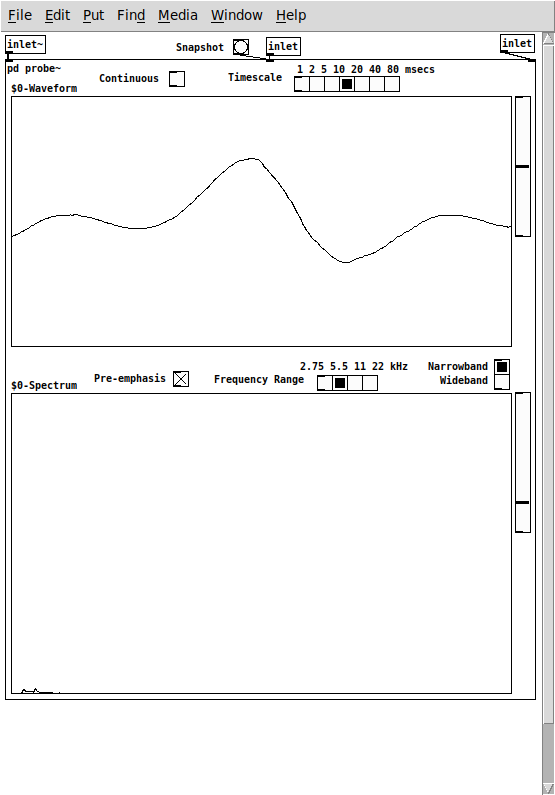
\includegraphics[width=0.6\textwidth]{question1.png}}
  \end{center}
\end{figure}
\end{mdframed}
\vspace*{\baselineskip}

{\color{red}{\bfseries QUESTION \myq\  \emph{(worth up to 5 marks)}}\\Which sounds are most affected when the low-pass cut-off frequency is set to around 500 Hz - vowels or consonants - and why?}
\\
\begin{mdframed}
Consonants are most affected, particularly unvoiced sounds. As explained in question 1, unvoiced sounds use higher frequencies, which the low-pass filter nullifies. As vowels are all voiced, consonants are more heavily affected.
\end{mdframed}
\vspace*{\baselineskip}

{\color{red}{\bfseries QUESTION \myq\ \emph{(worth up to 5 marks)}}\\How is it that the speech is still quite intelligible when the high-pass cut-off frequency is set to 10 kHz?}
\\
\begin{mdframed}
Unvoiced sounds are not particularly affected by the high-pass filter at this setting because they primarily activate higher frequencies than the filter is capable of stopping. The pitch and tone of voiced sounds is also still intelligible - as can be observed with a narrowband filter spectrum, the frequencies that aren't cut off still display a variety of readings that shape the sound in spite of such a high cutoff point.
\end{mdframed}
\vspace*{\baselineskip}

{\color{red}{\bfseries QUESTION \myq\ \emph{(worth up to 5 marks)}}\\COM3502-4502-6502: The \texttt{[GraphicEqualiser$\sim$]} object uses an FFT internally; what does FFT stand for and what does an FFT do?\\COM4502-6502 ONLY: What is a DFT and how is it different from an FFT?}
\\
\begin{mdframed}
Replace this text with your answer.  Replace this text with your answer.  Replace this text with your answer.  Replace this text with your answer.  Replace this text with your answer.  Replace this text with your answer.  Replace this text with your answer.  Replace this text with your answer.  Replace this text with your answer.  Replace this text with your answer.  Replace this text with your answer.  Replace this text with your answer.  Replace this text with your answer.  Replace this text with your answer.  Replace this text with your answer.
FFT stands for Fast Fourier Transform. FFTs can be used to find the individual components at a frequency.
\end{mdframed}
\vspace*{\baselineskip}

{\color{red}{\bfseries QUESTION \myq\ \emph{(worth up to 10 marks)}}\\With \texttt{speed = 50} and \texttt{depth = 0.5}, what are the minimum and maximum amplitudes of your LFO output, and how do they vary with changes in these two settings?  Also, please provide two screenshots: (a) your \texttt{[LFO$\sim$-help]} object and (b) the internal structure of your \texttt{[LFO$\sim$]} object.}
\\
\begin{mdframed}
Replace this text with your answer.  Replace this text with your answer.  Replace this text with your answer.  Replace this text with your answer.  Replace this text with your answer.  Replace this text with your answer.  Replace this text with your answer.  Replace this text with your answer.  Replace this text with your answer.  Replace this text with your answer.  Replace this text with your answer.  Replace this text with your answer.  Replace this text with your answer.  Replace this text with your answer.  Replace this text with your answer.
\begin{figure}[H]
  \begin{center}
    \frame{
\includegraphics[width=0.6\textwidth]{screenshot.jpg}}
  \end{center}
\end{figure}
\begin{figure}[H]
  \begin{center}
    \frame{
\includegraphics[width=0.6\textwidth]{screenshot.jpg}}
  \end{center}
\end{figure}
\end{mdframed}
\vspace*{\baselineskip}

{\color{red}{\bfseries QUESTION \myq\ \emph{(worth up to 5 marks)}}\\In your own words\footnote{I.e.\ do not plagiarise from Wikipedia.}, why is this effect known as `ring modulation'?}
\\
\begin{mdframed}
Both amplitude modulation and ring modulation are multiplied by a carrier signal and a modulation signal. The difference is that the range of the modulation signal for amplitude modulation is between 0-1, which will cause the modulated signal to follow the modulation signal in amplitude. However, the modulation signal range of the ring modulation is between -1 and 1. After modulation, both the modulation signal and the carrier signal disappear, but the articulation is the same as the original input. Ring modulation is named because its circuit design is a ring.
\end{mdframed}
\vspace*{\baselineskip}

{\color{red}{\bfseries QUESTION \myq\ \emph{(worth up to 5 marks)}}\\Why is SSB commonly used in long-distance radio voice communications?}
\\
\begin{mdframed}
1. Saving the frequency band Because single-sideband communication uses only one sideband in the AM signal for communication, the frequency band can be saved. 2. Power saving. Reduced sideband and power loss.
\end{mdframed}
\vspace*{\baselineskip}

{\color{red}{\bfseries QUESTION \myq\ (\emph{worth up to 5 marks)}}\\COM3502-4502-6502: Why can the voice be shifted up in frequency much further than it can be shifted down in frequency before it becomes severely distorted?  \emph{Hint: look at \texttt{[wsprobe$\sim$]}.}\\COM4502-6502 ONLY: Your frequency shifter changes all the frequencies present in an input signal. How might it be possible to change the pitch of a voice \emph{without} altering the formant frequencies?}
\\
\begin{mdframed}
Replace this text with your answer.  Replace this text with your answer.  Replace this text with your answer.  Replace this text with your answer.  Replace this text with your answer.  Replace this text with your answer.  Replace this text with your answer.  Replace this text with your answer.  Replace this text with your answer.  Replace this text with your answer.  Replace this text with your answer.  Replace this text with your answer.  Replace this text with your answer.  Replace this text with your answer.  Replace this text with your answer.
\end{mdframed}
\vspace*{\baselineskip}

{\color{red}{\bfseries QUESTION \myq\ \emph{(worth up to 5 marks)}}\\In a practical system, why is it important to keep the feedback gain less than 1?}
\\
\begin{mdframed}
Replace this text with your answer.  Replace this text with your answer.  Replace this text with your answer.  Replace this text with your answer.  Replace this text with your answer.  Replace this text with your answer.  Replace this text with your answer.  Replace this text with your answer.  Replace this text with your answer.  Replace this text with your answer.  Replace this text with your answer.  Replace this text with your answer.  Replace this text with your answer.  Replace this text with your answer.  Replace this text with your answer.
\end{mdframed}
\vspace*{\baselineskip}

{\color{red}{\bfseries QUESTION \myq\ \emph{(worth up to 50 marks\footnote{25 for functionality, 15 for design/layout, 5 for \texttt{Pd} features, 5 for innovations})}}\\Please provide a short\footnote{no more than 500 words} description of the operation of your \texttt{[VoiceChanger]} application, together with a screenshot of your final GUI.}
\\
\begin{mdframed}
Replace this text with your answer.  Replace this text with your answer.  Replace this text with your answer.  Replace this text with your answer.  Replace this text with your answer.  Replace this text with your answer.  Replace this text with your answer.  Replace this text with your answer.  Replace this text with your answer.  Replace this text with your answer.  Replace this text with your answer.  Replace this text with your answer.  Replace this text with your answer.  Replace this text with your answer.  Replace this text with your answer.
\begin{figure}[H]
  \begin{center}
    \frame{
\includegraphics[width=0.6\textwidth]{screenshot.jpg}}
  \end{center}
\end{figure}
\end{mdframed}
\vspace*{\baselineskip}

\end{document}
